\documentclass[8pt]{beamer}
    \usepackage{graphicx}
    \usepackage{wrapfig}
    \usepackage{multicol}

    \usepackage[T1]{fontenc}
    \usepackage{mathptmx}
    \usetheme{Madrid}
    
    \title{IBD health}
    \author{Ahmed Ayman}
    
    \begin{document}
        \maketitle
        \begin{frame}{Agenda}
            \begin{itemize}
                \item Introduction
                \item Dataset
                \item Q1: show the age of participants and BMI
                \item Q2: Which type of IBD tends to have sufferers of a higher BMI?
                \item Q3: Which type of IBD has more sufferers that smoke or previously smoked?
                \item Q4: Which type of IBD has more cancer sufferers?
                \item Q5: Which type of IBD has more heart disease sufferers?
                \item Q6: Which age group is most affected by Ulcerative colitis (diagnosis type 2 in the dataset)
            \end{itemize}
        \end{frame}

        \begin{frame}{Introduction}
            I received a task asking me to analysis data for inflammatory bowel disease patients.\\
            The task asked me to answer some questions
            \begin{enumerate}
                \item show the age of participants and BMI
                \item Which type of IBD tends to have sufferers of a higher BMI?
                \item Which type of IBD has more sufferers that smoke or previously smoked?
                \item Which type of IBD has more cancer sufferers?
                \item Which type of IBD has more heart disease sufferers?
                \item Which age group is most affected by Ulcerative colitis (diagnosis type 2 in the dataset)
            \end{enumerate}
        \end{frame}

        \begin{frame}{Dataset}
            The data contains information about 33K patients The data columns as follow
            \begin{itemize}
                \item pt-ID: unique ID for each patient
                \item gender: integer value indicates the gender of each patient
                    \begin{itemize}
                        \item 1 means male
                        \item 2 means female
                    \end{itemize} 
                \item diagnosis: integer value indicates the type of IBD
                    \begin{itemize}
                        \item 1 means Crohn's
                        \item 2 means UC
                        \item 3 means Unspecified
                        \item 4 means Other
                    \end{itemize}
                \item hosp-admin: integer value indicates if the patient recorded in a hospital or not
                \item age-band-jan1: the age value for each patient
                \item bmi: contains the body mass for each patient
                \item smoker: is the patient smoker or not
                \item past-smoker: is the patient was smoker or not
                \item diet-preference: which diet the patient follows
                \item cancer: is the patient has cancer or not
                \item heart-disease: is the patient has heart disease or not
            \end{itemize}
        \end{frame}

        \begin{frame}{Q1: show the age of participants and BMI}
            Please keep in mind this is just a \textbf{descriptive statistics}
            \centering
            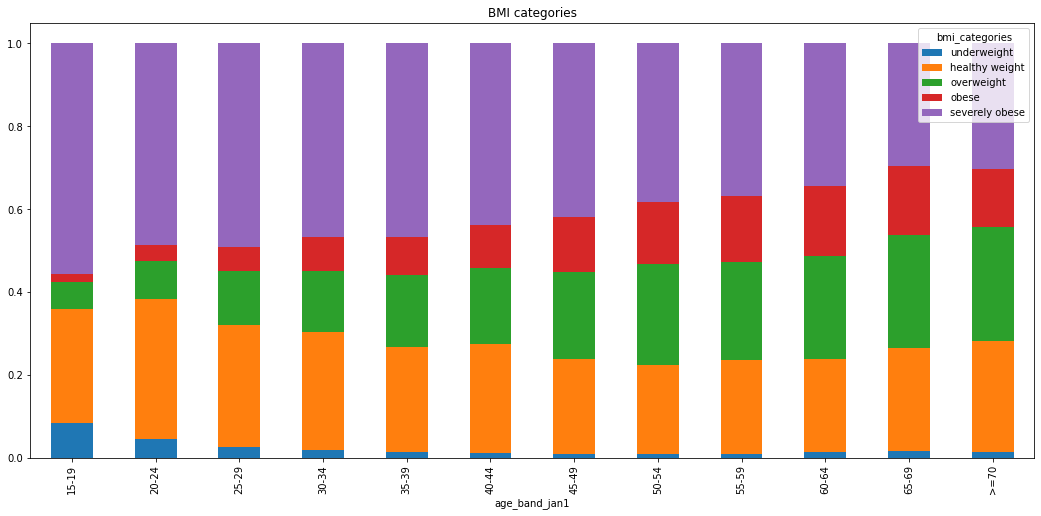
\includegraphics[width=.9\textwidth]{images/age-bmi.png}\\
            Just understand the data, but \textbf{\textcolor{red}{don't}} make any conclusions
        \end{frame}

        \begin{frame}{Q2: Which type of IBD tends to have sufferers of a higher BMI?}
            \textbf{IBD types}:-
            \begin{itemize}
                \item 1 means Crohn's
                \item \textcolor{blue}{2 means UC}
                \item 3 means Unspecified
                \item 4 means Other
            \end{itemize}
            \begin{center}
                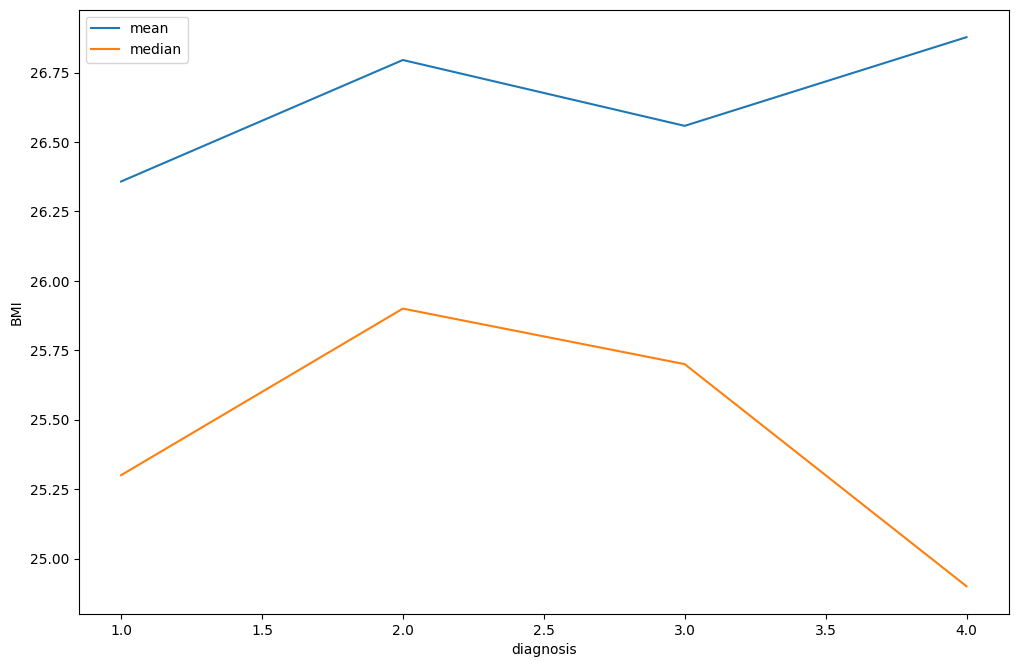
\includegraphics[height=.55\textheight]{images/BMI-IBD.png}\\
                Type 2 (UC): has the BMI\\
                Type 4: effect by outliers
            \end{center}
        \end{frame}

        \begin{frame}{Q3: Which type of IBD has more sufferers that smoke or previously smoked?}
            \textbf{IBD types}:-
            \begin{itemize}
                \item 1 means Crohn's
                \item 2 means UC
                \item 3 means Unspecified
                \item \textcolor{blue}{4 means Other}
            \end{itemize}
            \begin{center}
                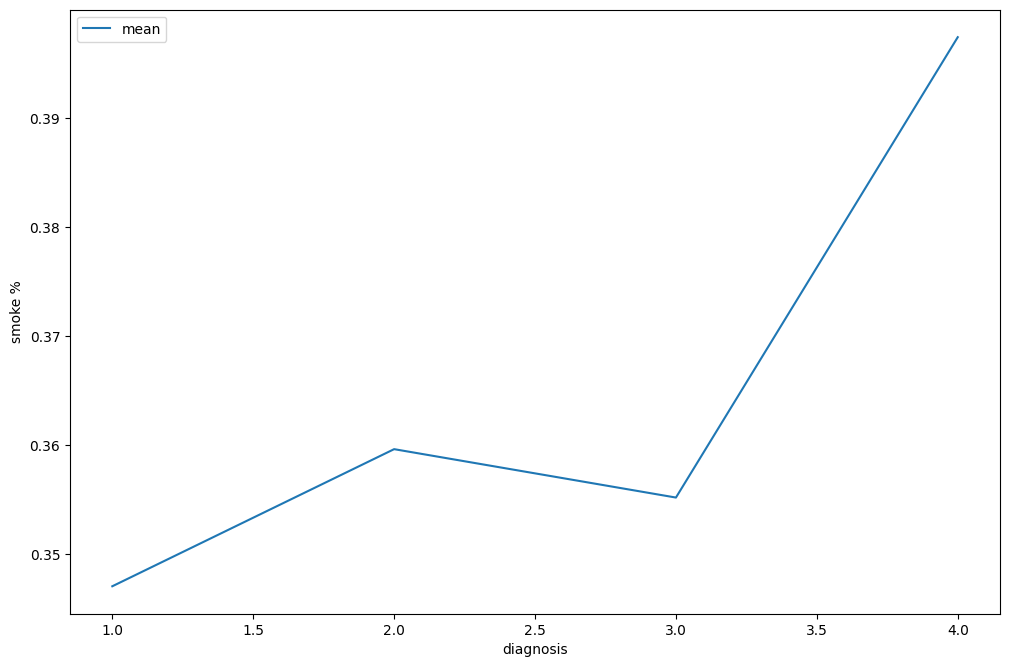
\includegraphics[height=.55\textheight]{images/smoke.png}\\
                Type 4: has the highest smoking percentage
            \end{center}
        \end{frame}

        \begin{frame}{Q4: Which type of IBD has more cancer sufferers?}
            \textbf{IBD types}:-
            \begin{itemize}
                \item 1 means Crohn's
                \item 2 means UC
                \item \textcolor{blue}{3 means Unspecified}
                \item 4 means Other
            \end{itemize}
            \begin{center}
                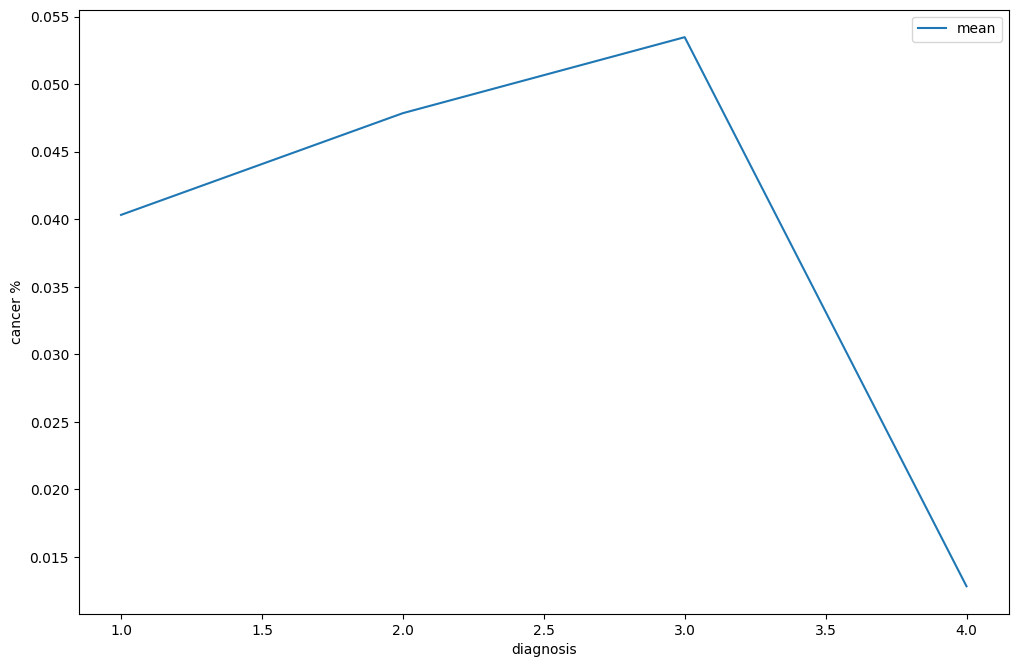
\includegraphics[height=.55\textheight]{images/cancer.png}\\
                Type 3: has the highest cancer percentage
            \end{center}
        \end{frame}

        \begin{frame}{Q5: Which type of IBD has more heart disease sufferers?}
            \textbf{IBD types}:-
            \begin{itemize}
                \item 1 means Crohn's
                \item \textcolor{blue}{2 means UC}
                \item 3 means Unspecified
                \item 4 means Other
            \end{itemize}
            \begin{center}
                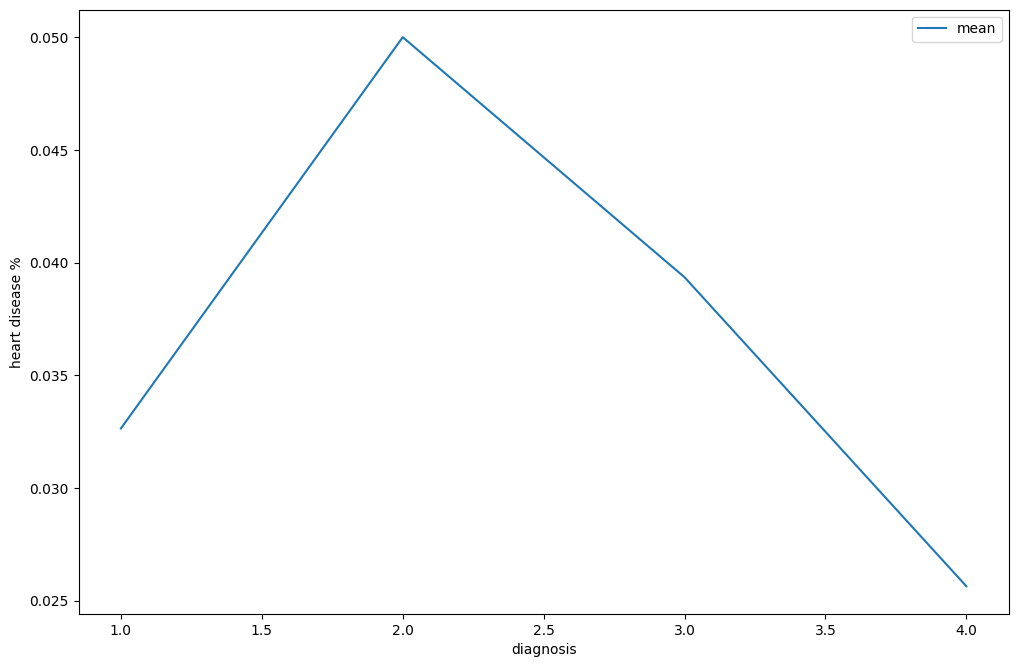
\includegraphics[height=.55\textheight]{images/heart.png}\\
                Type 2: has the highest heart disease percentage
            \end{center}
        \end{frame}

        \begin{frame}{Q6: Which age group is most affected by Ulcerative colitis?}
            \textbf{gender types}:-
            \begin{itemize}
                \item 1 means Male
                \item 2 means Female
            \end{itemize}
            \begin{center}
                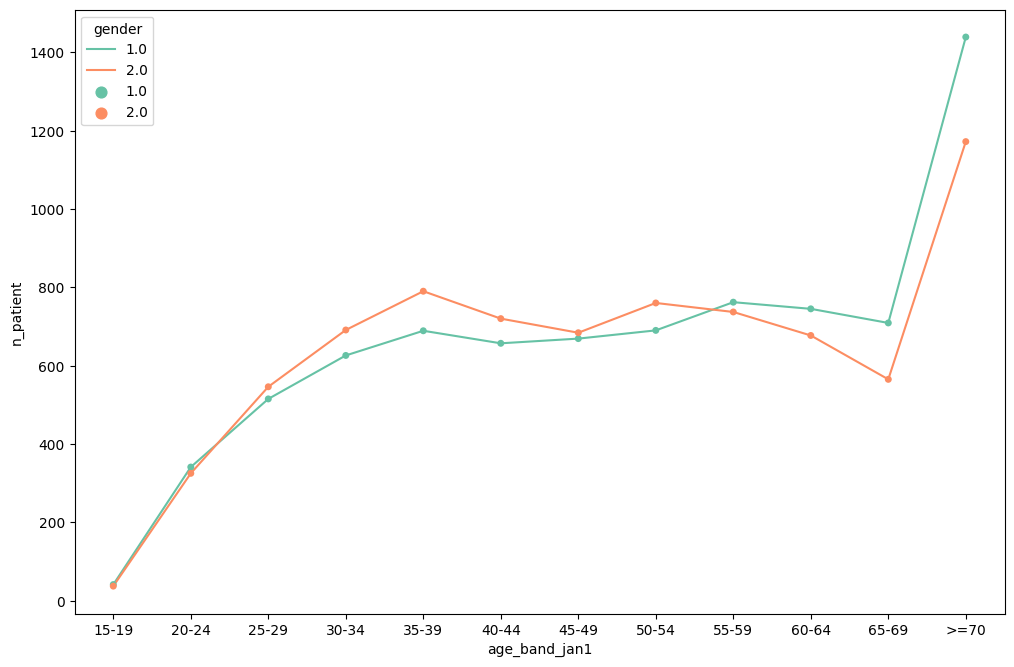
\includegraphics[height=.75\textheight]{images/uc-age.png}\\
            \end{center}
        \end{frame}
    \end{document}